\documentclass{article}

\usepackage{fancyhdr}
\usepackage{extramarks}
\usepackage{amsmath}
\usepackage{amsthm}
\usepackage{amsfonts}
\usepackage{tikz}
\usepackage[plain]{algorithm}
\usepackage{algpseudocode}
\usepackage{graphicx}
\usepackage{csquotes}
\usepackage{caption}
\usepackage{subcaption}
\usepackage{hyperref}
\hypersetup{
    colorlinks=true,
    linkcolor=blue,
    filecolor=blue,
    urlcolor=blue
}

\usetikzlibrary{automata,positioning}

%
% Basic Document Settings
%

\topmargin=-0.45in
\evensidemargin=0in
\oddsidemargin=0in
\textwidth=6.5in
\textheight=9.0in
\headsep=0.25in

\linespread{1.1}

\pagestyle{fancy}
\lhead{\hmwkAuthorName}
\chead{\hmwkClass\ (\hmwkClassInstructor): \hmwkTitle}
\rhead{\firstxmark}
\lfoot{\lastxmark}
\cfoot{\thepage}

\renewcommand\headrulewidth{0.4pt}
\renewcommand\footrulewidth{0.4pt}

\setlength\parindent{0pt}

%
% Create Problem Sections
%

\newcommand{\enterProblemHeader}[1]{
    \nobreak\extramarks{}{Problem \arabic{#1} continued on next page\ldots}\nobreak{}
    \nobreak\extramarks{Problem \arabic{#1} (continued)}{Problem \arabic{#1} continued on next page\ldots}\nobreak{}
}

\newcommand{\exitProblemHeader}[1]{
    \nobreak\extramarks{Problem \arabic{#1} (continued)}{Problem \arabic{#1} continued on next page\ldots}\nobreak{}
    \stepcounter{#1}
    \nobreak\extramarks{Problem \arabic{#1}}{}\nobreak{}
}

\setcounter{secnumdepth}{0}
\newcounter{partCounter}
\newcounter{homeworkProblemCounter}
\setcounter{homeworkProblemCounter}{1}
\nobreak\extramarks{Problem \arabic{homeworkProblemCounter}}{}\nobreak{}

%
% Homework Problem Environment
%
% This environment takes an optional argument. When given, it will adjust the
% problem counter. This is useful for when the problems given for your
% assignment aren't sequential. See the last 3 problems of this template for an
% example.
%
\newenvironment{homeworkProblem}[1][-1]{
    \ifnum#1>0
        \setcounter{homeworkProblemCounter}{#1}
    \fi
    \section{Problem \arabic{homeworkProblemCounter}}
    \setcounter{partCounter}{1}
    \enterProblemHeader{homeworkProblemCounter}
}{
    \exitProblemHeader{homeworkProblemCounter}
}

%
% Homework Details
%   - Title
%   - Due date
%   - Class
%   - Section/Time
%   - Instructor
%   - Author
%

\newcommand{\hmwkTitle}{Assignment\ \#6}
\newcommand{\hmwkDueDate}{December 1, 2020}
\newcommand{\hmwkClass}{SCI 238}
\newcommand{\hmwkClassInstructor}{Dr. Michael Fich}
\newcommand{\hmwkAuthorName}{\textbf{Zach Bortoff}}

%
% Title Page
%

\title{
    \vspace{2in}
    \textmd{\textbf{\hmwkClass:\ \hmwkTitle}}\\
    \normalsize\vspace{0.1in}\small{Due\ on\ \hmwkDueDate\ at 11:59pm}\\
    \vspace{0.1in}\large{\textit{\hmwkClassInstructor}}
    \vspace{3in}
}

\author{\hmwkAuthorName}
\date{}

\renewcommand{\part}[1]{\textbf{\large Part \Alph{partCounter}}\stepcounter{partCounter}\\}

%
% Various Helper Commands
%

% Useful for algorithms
\newcommand{\alg}[1]{\textsc{\bfseries \footnotesize #1}}

% For derivatives
\newcommand{\deriv}[1]{\frac{\mathrm{d}}{\mathrm{d}x} (#1)}

% For partial derivatives
\newcommand{\pderiv}[2]{\frac{\partial}{\partial #1} (#2)}

% Integral dx
\newcommand{\dx}{\mathrm{d}x}

% Alias for the Solution section header
\newcommand{\solution}{\textbf{\large Solution}}

% Probability commands: Expectation, Variance, Covariance, Bias
\newcommand{\E}{\mathrm{E}}
\newcommand{\Var}{\mathrm{Var}}
\newcommand{\Cov}{\mathrm{Cov}}
\newcommand{\Bias}{\mathrm{Bias}}

\begin{document}

\maketitle

\pagebreak

\begin{homeworkProblem}
    \textbf{Solution}

	(a.)\\
	\begin{figure}[!h]
		\centering
		\textbf{Figure 1: Table of Galactic Data}\\
		\begin{tabular}{rrr}
			\hline\hline
			\textbf{Distance} & \textbf{Velocity} & \textbf{Mass} \\
			\texttt{kpc} & \texttt{km/s} & \texttt{kg} \\\hline
			5.0 & 245.0 & \(1.388\times 10^{41}\) \\
			10.0 & 270.0 & \(3.37\times 10^{41}\) \\
			15.0 & 260.0 & \(4.688\times 10^{41}\) \\
			20.0 & 270.0 & \(6.741\times 10^{41}\) \\
			25.0 & 265.0 & \(8.117\times 10^{41}\) \\\hline\hline
		\end{tabular}
		\caption{Table of galactic radial distance, velocity, and mass. Velocities were estimated using the graph in the assignment. A sample mass calculation can be found below.}
	\end{figure}\\
	
	Sample Mass Calculation (\(R=5\hspace{3pt}[kpc]\), \(v\approx 245.0\hspace{3pt} [km/s]\))
	\[
		v_{circ}^2 = \frac{G M_R}{R}
		\Longleftrightarrow M_R = \frac{R v_{circ}^2}{G} = \frac{(5\hspace{3pt} [kpc])(245.0\hspace{3pt}[km/s])^2)}{6.67408\times 10^{-11} \hspace{3pt} [m^3kg^{-1}s^{-2}]}\approx 1.388 \times 10^{41} \hspace{3pt}[kg]
	\]\\
	(b.)\\
	\begin{figure}[!h]
		\centering
		\textbf{Figure 2: Log-log Plot of Galactic Mass vs. Radial Distance}\\
		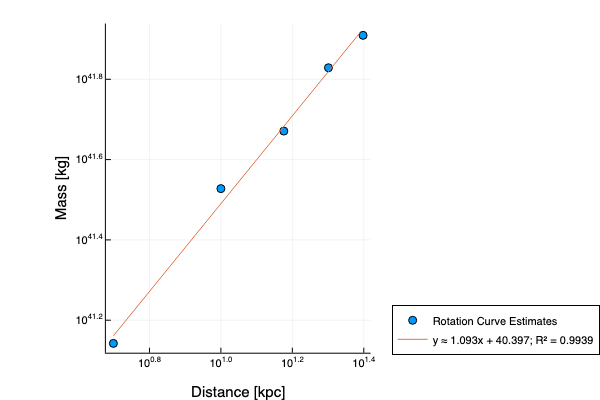
\includegraphics[width=0.75\linewidth]{GalacticMassVSRadialDist.png}
		\caption{Log-log plot of Galactic Mass versus Radial Distance. The blue points represent the data from Figure 1. The line-of-best fit (as computed using Least-Squares algorithm) is the orange line. }
	\end{figure}\\
	
	(c.) To compute \(\rho_0\) and \(\alpha\), we must first take the \(log\) of both sides of \(M_r = 4\pi \rho_0 R^{3-\alpha}\), which yields: \( (1) \rightarrow log_{10}(M_r) = log_{10}(4\pi \rho_0) + (3-\alpha)log_{10}(R)\).\\
	
	Our goal is to match equation \((1)\) to the equation for the line-of-best fit found in the previous section (i.e. the equation for a line). 
	
	\[
		b = log_{10}(4\pi \rho_0) \Longleftrightarrow \rho_0 = \frac{10^b}{4\pi}\approx \frac{10^{40.40}}{4\pi}\approx 1.98\times 10^{39} \hspace{3pt} [kg]
	\]
	\[
		m = 3 - \alpha \Longleftrightarrow \alpha = 3 - m \approx 3 - 1.09 \approx 1.91 \hspace{3pt} [kg/kpc]
	\]
\end{homeworkProblem}

\pagebreak


\begin{homeworkProblem}
 	2) Determine the age of a Universe where the data in the table below were measured for a set
of galaxies, all appear relatively close together in the sky. (a) Make a Hubble Diagram of this data.
(b) Estimate the age from this data for the “open” or “unbound” cosmological model with
constant expansion (i.e. constant velocity, no net acceleration). (c) You may have noticed that the
intercept of the plot is not zero. Why would this happen? (d) Determine the age if the Universe is
“flat” (i.e. on the boundary between “open” and “closed” or between “unbound” and “bound”).
(Marks: 5) \textit{(Note: this is NOT our Universe!)} \\
 	
 	\textbf{Solution}
 	
 	(a.)
 	\begin{figure}[!h]
		\centering
		\textbf{Figure 3: Hubble Diagram}\\
		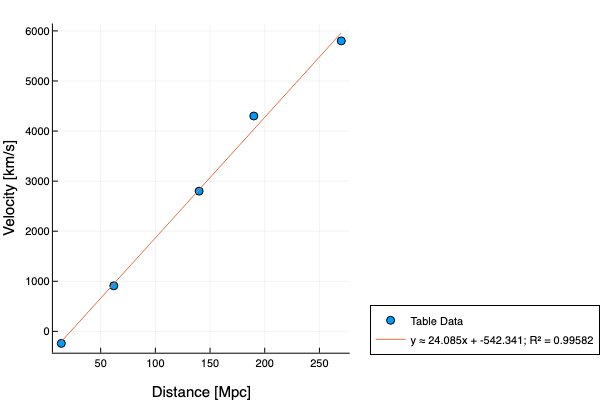
\includegraphics[width=0.75\linewidth]{HubbleDiagram.png}
		\caption{Hubble Diagram of sample data. The blue points represent the data in the table given in the assignment. The line-of-best fit (as computed using Least-Squares algorithm) is the orange line. }
	\end{figure}\\
	
	(b.) The Empty age of the universe can be computed by taking the inverse of the Hubble constant, which corresponds with slope of the line-of-best fit in Figure 3. Let \(a_e\) denote the empty age:
	
	\[
		H_0 = m \approx 24.09 \hspace{3pt} [km/s/Mpc]
	\]
	\[
		a_e = 1 / H_0 \approx 40.6 \hspace{3pt} [billion\hspace{3pt} years]
	\]
	
	(c.) There are multifarious reasons for the intercept of this line not being exactly zero. For one, one of the points in our data set - in fact the galaxy closest to us - has a negative velocity. This suggests that that galaxy is travelling towards us - perhaps it's orbiting another galaxy, perhaps we're on a collision course with that galaxy. Whatever the case may be, we know that the contribution due to the expansion of the universe to the velocity of another galaxy is smaller for galaxies closer to us. Therefore, for nearby galaxies, the noise introduced to measurements of radial velocity due to other sources of velocity - such as orbits around a third galaxy or gravity bringing our two galaxies together - has a much more significant impact on the overall measurement. \\
	On the other extreme, velocity and distance measurements of galaxies are particularly difficult to accurately measure - especially as those galaxies get further and further away from us. So uncertainties introduced from imprecise measurements of distant galaxies could also be affecting our ability to ascertain a line-of-best fit whose y-intercept is zero.\\
	
	(d.) The Flat age of the universe, denoted by \(a_f\) can be computed by multiplying the empty age by \(2/3\). 
	
	\[
		a_f = \frac{2}{3H_0} \approx 27.1 \hspace{3pt} [billion\hspace{3pt} years]
	\]
	
\end{homeworkProblem}

\pagebreak

\end{document}
